% !TEX root = Tesi.tex
\chead{}

\chapter{Enhancing web models via model transformations}
\label{enhancing-web-models-via-model-transformations}

\section{Transformation}

In the last chapter, after describing both metamodels for the Real Usage Data and the Interaction Flow Modeling Language,  we proceeded to create dynamic instances for both models respectively describing the actual input data available for the personalization process and the initial IFMLModel of the eCommerce Madison Island website. In this chapter, we illustrate a possible model transformation for this model based on the Real Usage instance data with the goal of creating an upgraded model version which takes into account the customer preferences and his actions.

\subsection{Homepage}
\label{homepage-updates}
Considering the data coming from the Proximity sensors within the actual Madison Island retail store we are aware of a set of regions corresponding to the categories the user prefers over the others, this information will be used to change the content, and therefore the IFMLModel, for the Homepage carousel.

For instance, we know that \textbf{Blazers},\textbf{Tees, Knits and Polos} and \textbf{Shoes} categories correspond to the \textit{sessionRegion} elements where the user spent more time within the store after sorting the entries by \textit{maxSecondsInRegion} and \textit{maxProximity}. In the case of the Blazers category for example, the data belonging to the \textit{RealUsageData:ProximityData} parent node has this form:

\vspace{0.5cm}
\lstset{language=XML}
\begin{lstlisting} 
  <sessionRegions
  regionId="40"
  regionLabel="blazers"
  detectionCount="1"
  maxSecondsInRegion="195"
  maxProximity="immediate"
  firstDetectionTimeStamp="2018-02-21T18:11:01.000+0100"
  lastDetectionTimeStamp="2018-02-21T18:11:01.000+0100">
  <beaconData
    uuid="0686a88e-fed6-11e7-8be5-0ed5f89f718b"
    majorId="25911"
    minorId="27"/>
</sessionRegions>
\end{lstlisting}
\vspace{0.5cm}

Applying this knowledge, the \textit{subViewComponentParts} and the \textit{parameter} nodes of the first HightlightedCategoriesCarousel \textit{IFMLWindow} elements from the initial \textit{IFMLModel} can be modified from this:

\vspace{0.5cm}
\lstset{language=XML}
\begin{lstlisting} 
<parameters  name="Highlighted Category #1" direction="inout">
  <constraints  language="SQL" body="Category.ID=18"/>
</parameters>

...

<subViewComponentParts xsi:type="core:ConditionalExpression"  language="SQL" body="Category.ID=18" name="Eyewear"/>
\end{lstlisting}
\vspace{0.5cm}

to :

\vspace{0.5cm}
\lstset{language=XML}
\begin{lstlisting} 
  <parameters  name="Highlighted Category #1" direction="inout">
  <constraints  language="SQL" body="Category.ID=40"/>
</parameters>

...

<subViewComponentParts xsi:type="core:ConditionalExpression"  language="SQL" body="Category.ID=40" name="Blazers"/>
\end{lstlisting}
\vspace{0.5cm}

Besides this content update which priorities some categories over the others, the \textit{IFMLModel} can also be transformed to use different IFML elements under certain conditions. For example, the viewComponent which is responsible for displaying the most recent products on the homepage can be swapped with another \textit{List View Component} responsible for presenting the latest products the customer interacted with in the physical retail store. The information about these products is available in the RealUsageData model under the \textit{RealUsageData:ActionData} section and, in our specific example, it carries the data about the product SKUs the customer scanned with his smartphone camera to collect reward points.

\vspace{0.5cm}
\lstset{language=XML}
\begin{lstlisting} 
<sessionActions userAgent="iPhone 6S">
  <scannedItems 
  barcode="042100005264" name="Elizabeth Knit Top-Red-S" sku="wbk012c-Red-S"/>
  <scannedItems 
  barcode="042100005931" name="Plaid Cotton Shirt-Khaki-L" sku="msj006c-Khaki-L"/>
  <scannedItems 
  barcode="042100007717" name="Broad St Saddle Shoes" sku="shm00110"/>
</sessionActions>
\end{lstlisting}
\vspace{0.5cm}


The model transition in this case would occurr not only replacing the IFML viewComponent with a different type but also adding a \textit{ConditionalExpression} filtering the items by their SKUs as per shown in Figure \ref{fig:ifml-transformation-example}.

\vspace{0.5cm}
\begin{figure}[H]
  \centering
    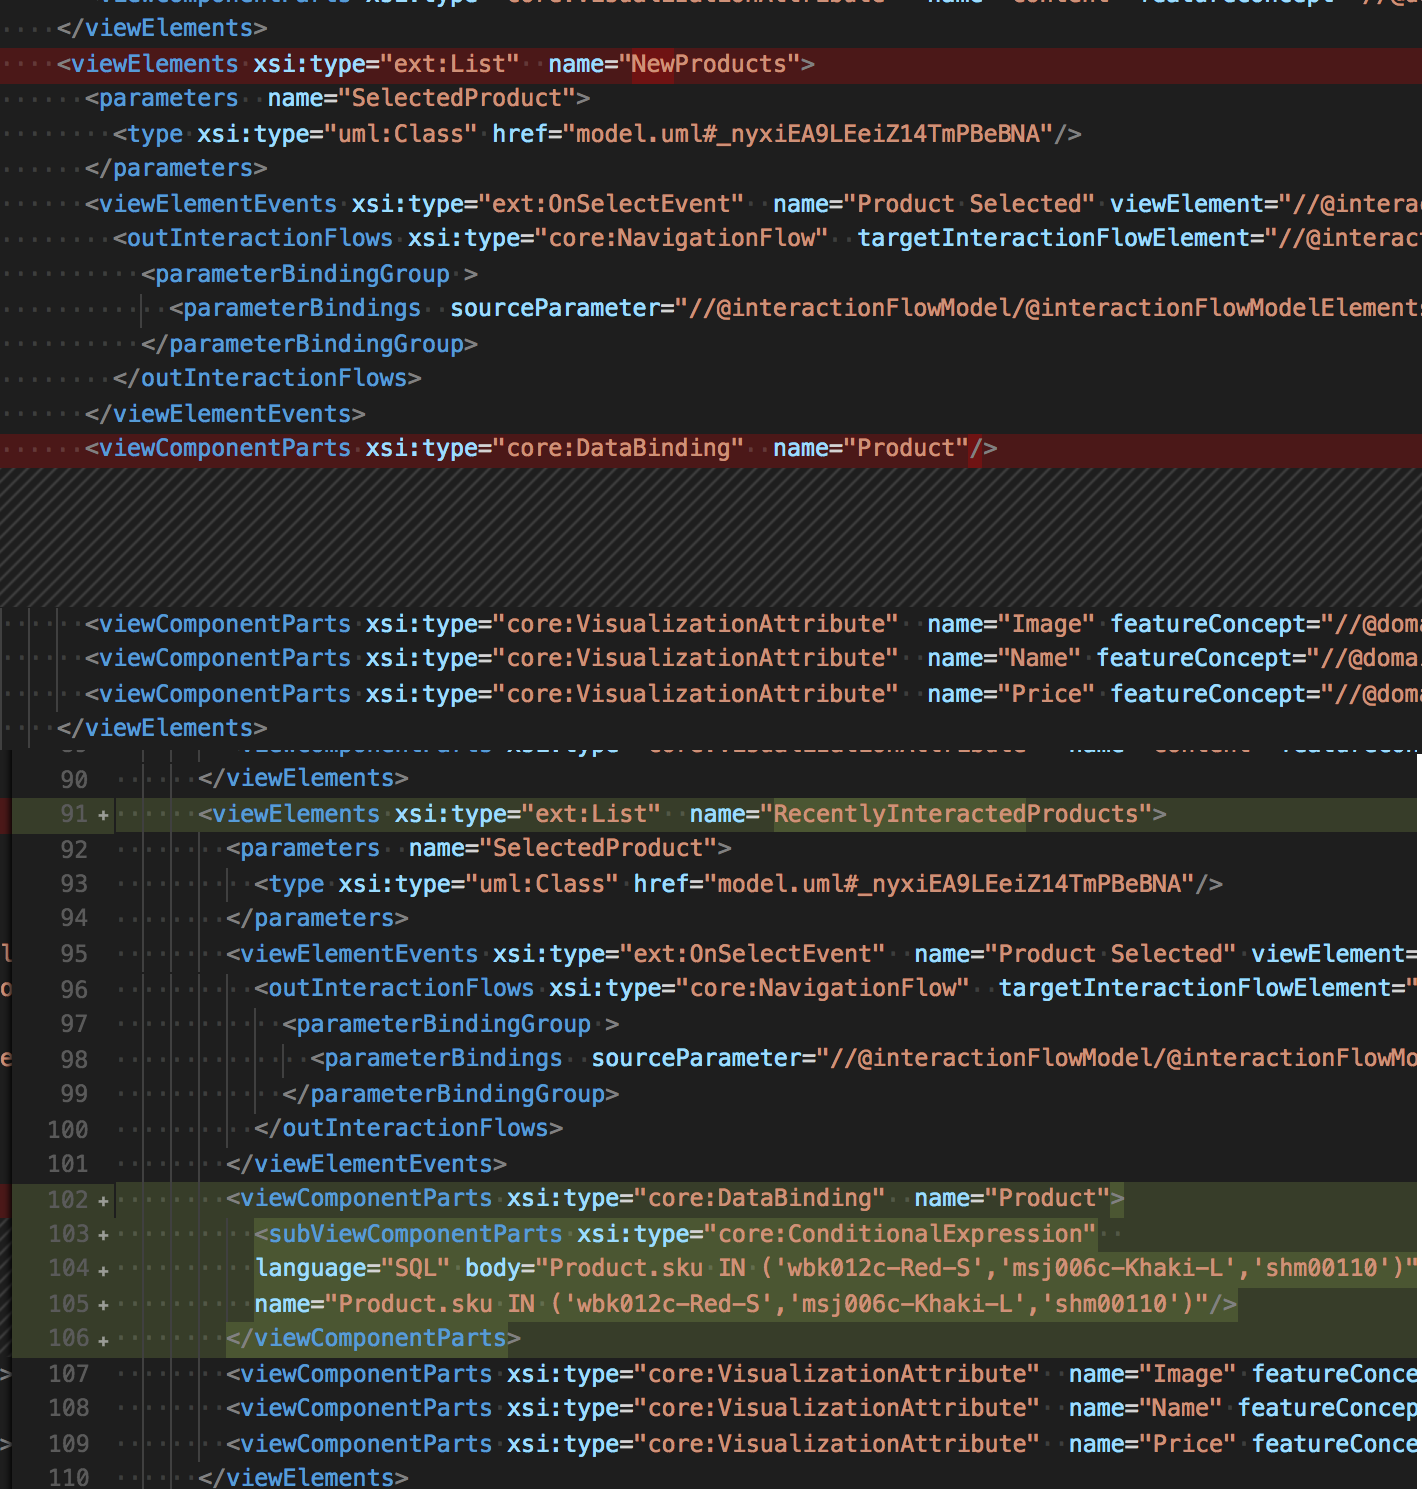
\includegraphics[height=12cm]{images/madison/ifm-homepage-transformation.png}
  \caption{IFML Homepage transformation example}
  \label{fig:ifml-transformation-example}
\end{figure}
\vspace{0.5cm}

\subsection{Header}
\label{header-updates}
Leveraging once more the \textit{RealUsageData:ActionData}, the Header node of the IFMLModel describing the Madison Island website top area could also be enhanced to show a list of recent actions which generated reward points performed by the customer in the physical stores.  This is achieved appending  an instance of \textit{List View Component} to the \textit{interactionFlowModelElements} parent node called \textit{RecentRewardActions} linked to the Rewards \textit{Data Binding} entity and visualizing the \textit{Action Name} and \textit{Points Attribution} properties to the frontend as per shown in the following snippet of code of the \textit{IFMLModel}:

\vspace{0.5cm}
\lstset{language=XML}
\begin{lstlisting} 
  <interactionFlowModelElements xsi:type="ext:IFMLWindow"  name="Header" isLandmark="true">
  <viewElements xsi:type="ext:List"  name="NavigationMenu">
   ...
  </viewElements>
  <viewElements xsi:type="ext:Form"  name="SearchForm">
   ...
  </viewElements>
  <viewElements xsi:type="core:ViewComponent"  name="TopLinks"/>
  <viewElements xsi:type="core:ViewComponent"  name="LanguageSwitch"/>

  <!-- ADDED NODE -->
  <viewElements xsi:type="ext:List"  name="RecentRewardActions">
    <viewComponentParts xsi:type="core:DataBinding"  name="Rewards" domainConcept="//@domainModel/@domainElements.13"/>
    <viewComponentParts xsi:type="core:VisualizationAttribute"  name="Action Name" featureConcept="//@domainModel/@domainElements.15"/>
    <viewComponentParts xsi:type="core:VisualizationAttribute"  name="Points Attribution" featureConcept="//@domainModel/@domainElements.14"/>
  </viewElements>
  <!-- ADDED NODE -->

  </interactionFlowModelElements>
\end{lstlisting}
\vspace{0.5cm}

\subsection{Category Page}
\label{category-page-updates}
In light of the information gathered in the Real Usage Data model about the recently viewed products available in the \textit{RealUsageData:WebData} node, the Category page can be enhanced appending an additional visual element to the user interface to track this information.

To do so, we filter out the RealUsageData model fetching the nodes containing a \textit{parameterBindingGroup} property including a Product reference like the following entries :

\vspace{0.5cm}
\lstset{language=XML}
\begin{lstlisting} 
      <data xsi:type="RealUsageData:WebData"
      ID="3"
      name="AccessLog"
      userID="3045678"
      date="2017-11-29T07:08:40.000+0100"
      viewContainer="Category #15"
      viewComponent="ProductList"
      eventType="click"
      parameterBindingGroup="Product/404"
      logEntry="GET /men/shirts/plaid-cotton-shirt-476.html 200 0 - 29505"/>
      
      <data xsi:type="RealUsageData:WebData"
      ID="4"
      name="AccessLog"
      userID="3045678"
      date="2017-12-04T06:37:15.000+0100"
      viewContainer="Product #404"
      viewComponent="RelatedProductList"
      eventType="click"
      parameterBindingGroup="Product/413"
      logEntry="GET /core-striped-sport-shirt-551.html 200 0 - 29505"/>

      <data xsi:type="RealUsageData:WebData"
      ID="8"
      name="AccessLog"
      userID="3045678"
      date="2017-12-04T06:38:20.000+0100"
      viewContainer="Search Results"
      viewComponent="ProductList"
      eventType="click"
      parameterBindingGroup="Product/407"
      logEntry="GET /stretch-cotton-blazer-587.html 200 0 - 29505"/>
\end{lstlisting}
\vspace{0.5cm}

With the above data we can then proceed transforming the intial IFML Model for the Category page appending a \textit{RecentlyViewedProducts} section in the form of a \textit{List View Component} bound to the Product \textit{Data Binding} entity.

This new IFML item would be responsible for presenting the thumbnails, names and prices of these products to the customer separating them through a distinct \textit{ConditionalExpression} which maps the children node of the \textit{RealUsageData:WebData} dataset shown earlier before finally returning the items in the order they were browsed regardless of the display mode property of the Category itself (Figure \ref{fig:recently-viewed-ifml-definition}).

\vspace{0.5cm}
\begin{figure}[H]
  \centering
    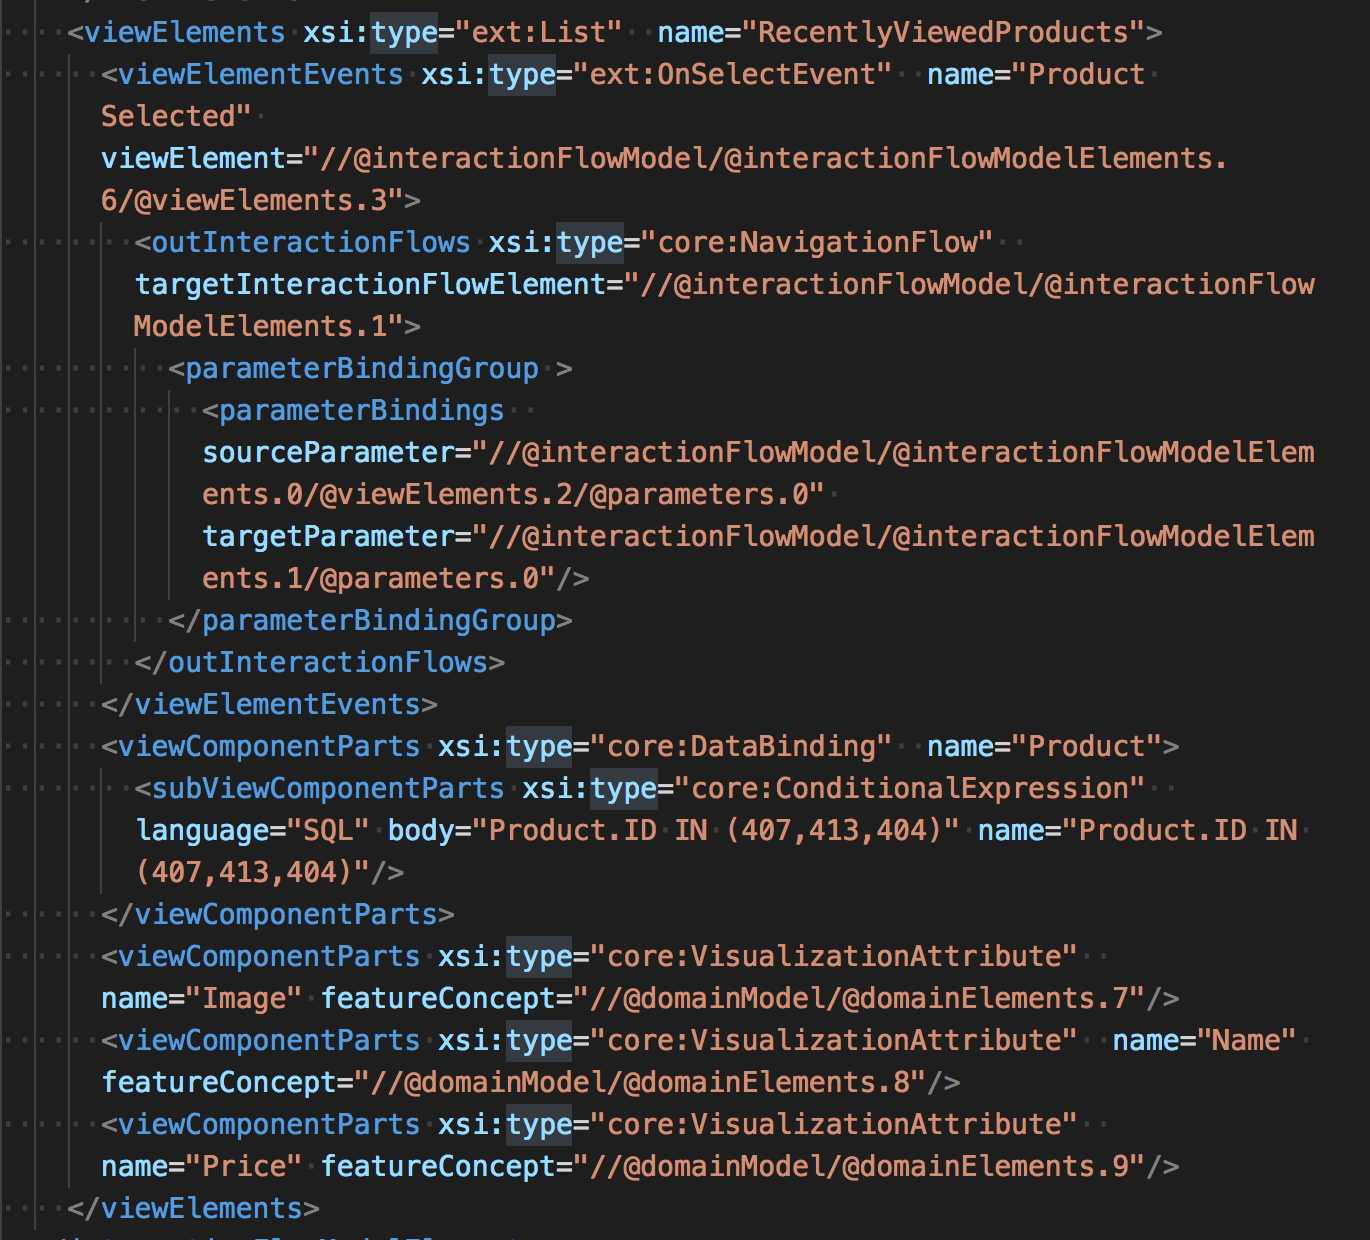
\includegraphics[height=12cm]{images/madison/ifml-recently-viewed.png}
  \caption{Recently Viewed IFML definition snippet}
  \label{fig:recently-viewed-ifml-definition}
\end{figure}
\vspace{0.5cm}

\subsection{Product Page}
\label{product-page-updates}

For what it involves the possible improvements on the product page of the Madison Island website, we concentrated on the Related Products widget shown just below the Add To Cart section. In the first \textit{IFMLModel} the list of the products related to the currently shown one has no particular logic assigned, our potential transformation can extend the \textit{viewElements} node of the \textit{IFMLModel} taking into consideration the browsing pattern of the users which have been identified examining the RealUsageData instances entries.

For example, we could have discovered that the \textbf{Core Striped Sport Shirt} product page is frequently browsed along with the \textbf{Plaid Cotton Shirt} product page during the same recorded sessions analyzing the values set in the \textit{viewContainer}, \textit{viewComponent} and \textit{parameterBindingGroup} properties for the nodes belonging to the \textit{RealUsageData:WebData} dataset. Due to this, we can take advantage of this correlation to push a product rather than another on the Related Products section for those products consequently offering a more tailored and customized experience to the user.

The transformation on the starting \textit{IFMLModel} that would occur in this case restricts the \textit{Data Binding} scope appending a \textit{subViewComponentParts} to it which limits the products collection to the computed set of related products SKUs. This additional \textit{ConditionalExpression} would also be bound to a specific \textit{ActivationExpression} which would enable the above filtering only when a customized collection for the current product is available. 

From a \textit{IFMLModel} code perspective, for the \textit{List View Component} which controls the Related Product widget we would transition from this node configuration :

\vspace{0.5cm}
\lstset{language=XML}
\begin{lstlisting} 
  <viewElements xsi:type="ext:List"  name="RelatedProductList">
  <viewElementEvents xsi:type="ext:OnSelectEvent"  name="Product Selected" viewElement="//@interactionFlowModel/@interactionFlowModelElements.1/@viewElements.2">
    ...
  </viewElementEvents>
  <viewComponentParts xsi:type="core:DataBinding"  name="Product"/>
  <viewComponentParts xsi:type="core:VisualizationAttribute"  name="Image" featureConcept="//@domainModel/@domainElements.7"/>
  <viewComponentParts xsi:type="core:VisualizationAttribute"  name="Name" featureConcept="//@domainModel/@domainElements.8"/>
  <viewComponentParts xsi:type="core:VisualizationAttribute"  name="Price" featureConcept="//@domainModel/@domainElements.9"/>
</viewElements>
\end{lstlisting}
\vspace{0.5cm}

to this one :

\vspace{0.5cm}
\lstset{language=XML}
\begin{lstlisting} 
  <viewElements xsi:type="ext:List"  name="RelatedProductList">
  <viewElementEvents xsi:type="ext:OnSelectEvent"  name="Product Selected" viewElement="//@interactionFlowModel/@interactionFlowModelElements.1/@viewElements.2">
      ...
  </viewElementEvents>
  <viewComponentParts xsi:type="core:DataBinding"  name="Product">
    <subViewComponentParts xsi:type="core:ConditionalExpression"  language="SQL" body="Product.ID IN getCustomizedRelatedProducts()" name="Product.ID IN getCustomizedRelatedProducts" activationExpression="//@interactionFlowModel/@interactionFlowModelElements.17"/>
  </viewComponentParts>
  <viewComponentParts xsi:type="core:VisualizationAttribute"  name="Image" featureConcept="//@domainModel/@domainElements.7"/>
  <viewComponentParts xsi:type="core:VisualizationAttribute"  name="Name" featureConcept="//@domainModel/@domainElements.8"/>
  <viewComponentParts xsi:type="core:VisualizationAttribute"  name="Price" featureConcept="//@domainModel/@domainElements.9"/>
</viewElements>
\end{lstlisting}
\vspace{0.5cm}

Moreover, the \textit{ActivationExpression} defined by the \textit{interactionFlowModelElements} XPath expression presented in the above snippet  links to a node responsible for the control of the feature with the following content:

\vspace{0.5cm}
\lstset{language=XML}
\begin{lstlisting} 
<interactionFlowModelElements 
  xsi:type="core:ActivationExpression" id="CurrentProduct.hasCustomizedRelatedProduct" language="SQL" body="CurrentProduct.hasCustomizedRelatedProduct()">
</interactionFlowModelElements>

\end{lstlisting}
\vspace{0.5cm}
\subsection{Shopping Cart}

As per described in \ref{shopping-cart-page-overview}, the Shopping Cart page model includes two main sections: a \textit{List Product List} component responsible for the interactions with the cart items and a \textit{IFMLWindow} for grouping the actions the customer may trigger through the interface for applying discounts or estimating shipping and taxes on his current quote.

\vspace{0.5cm}
\begin{figure}[H]
  \centering
    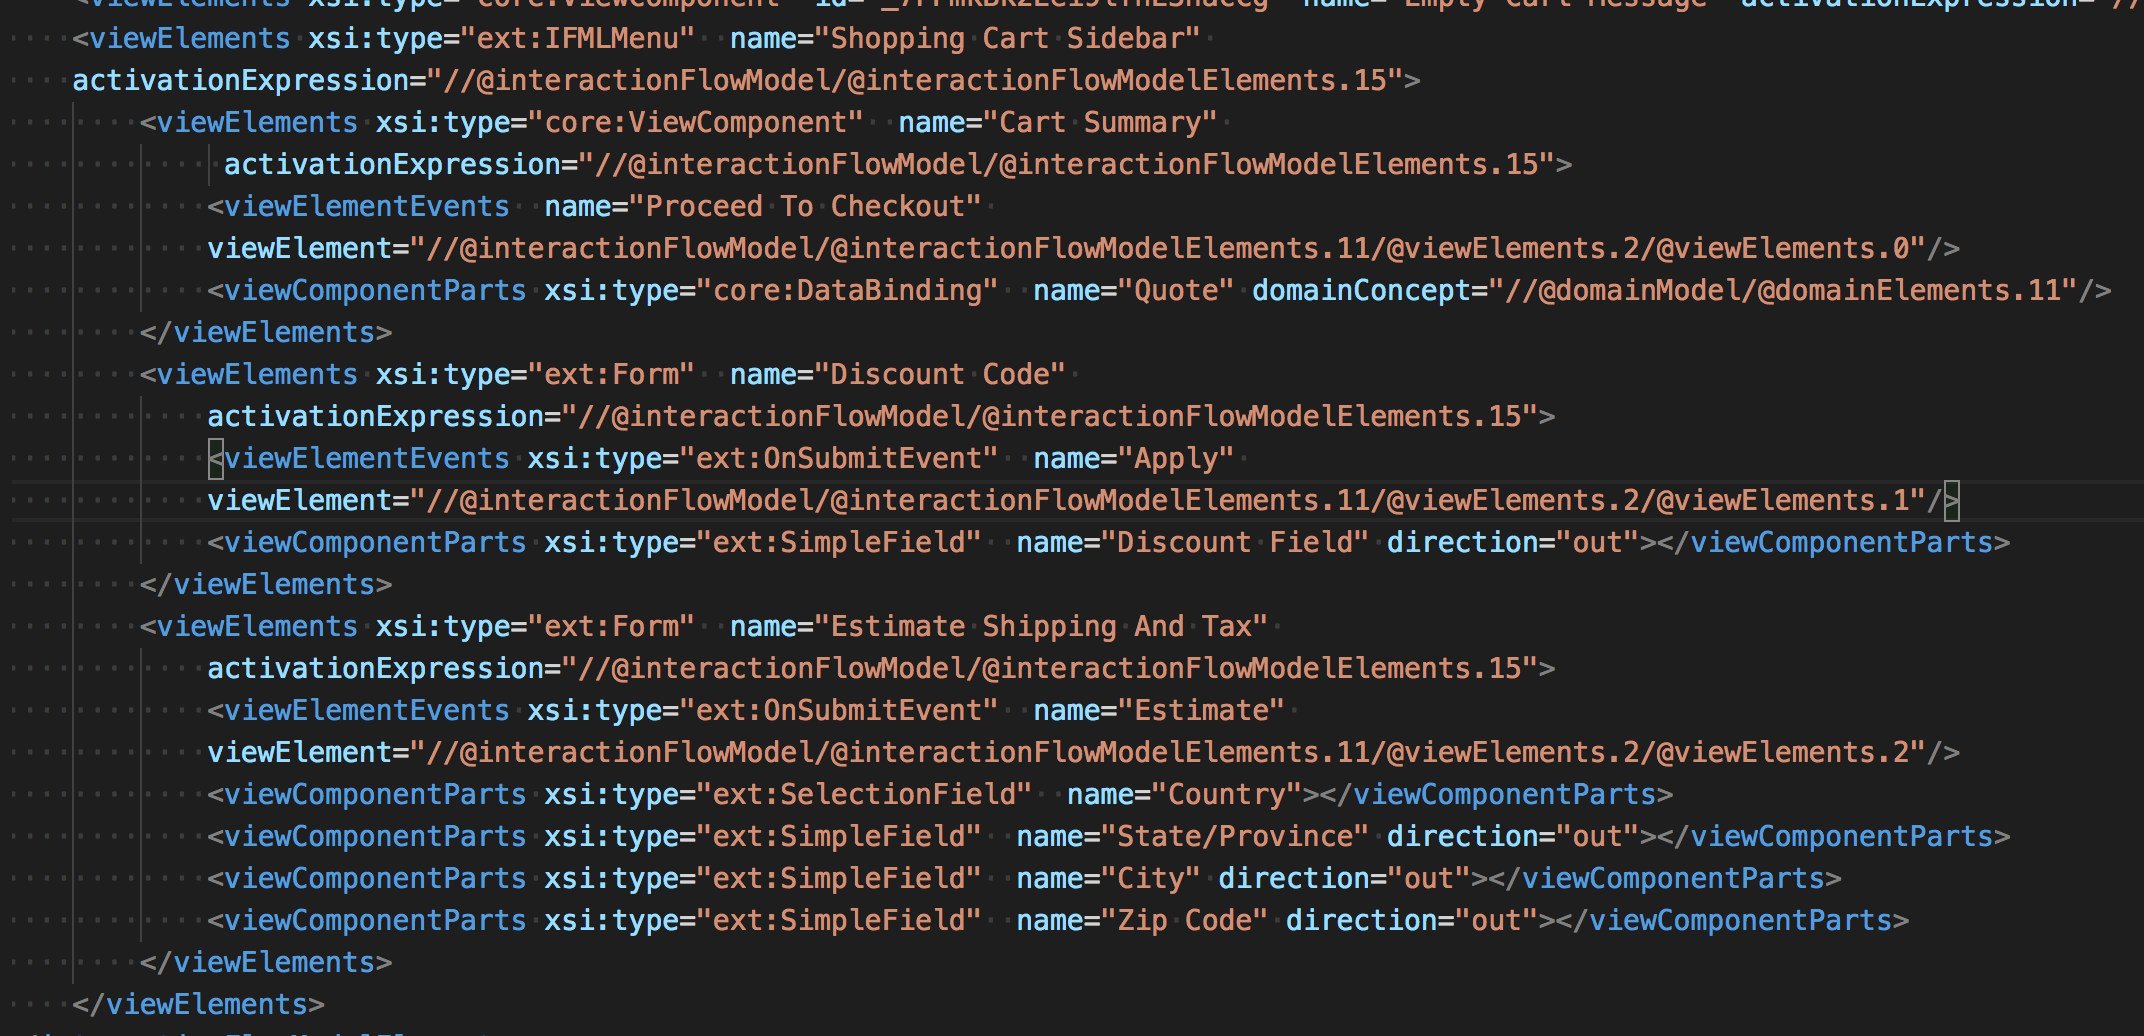
\includegraphics[width=12cm]{images/madison/ifml-shopping-cart-sidebar.png}
  \caption{Shopping Cart Sidebar IFML definition snippet}
  \label{fig:shopping-cart-sidebar-ifml-definition}
\end{figure}
\vspace{0.5cm}

Along with the previous analysed cases, applying the data from the Real Data Usage model, we can modify and extend the interaction flow of this page adding a brand new \textit{View Component} responsible for showing the Reward points the user accumulated within the Shopping Cart Sidebar (Figure \ref{fig:shopping-cart-sidebar-ifml-definition}). The component not only displays the information by the  \textit{Data Binding} with the Reward entity but it also controls the \textit{Event} associated with the \textbf{"Apply Discount"} button and the \textit{Action} connected to it. 
The structure of this new node which gets appended to its parent \textit{IFMLMenu} is the following :

\vspace{0.5cm}
\lstset{language=XML}
\begin{lstlisting} 
  <viewElements xsi:type="core:ViewComponent" name="Applicable Reward Points">
    <viewElementEvents xsi:type="ext:OnSelectEvent" name="Apply Reward Points" viewElement="//@interactionFlowModel/@interactionFlowModelElements.11/@viewElements.2/@viewElements.3">
        <outInteractionFlows xsi:type="core:NavigationFlow" targetInteractionFlowElement="//@interactionFlowModel/@interactionFlowModelElements.18/@actionEvents.0"/>
    </viewElementEvents>
    <viewComponentParts xsi:type="core:DataBinding" name="Reward"/>
    <viewComponentParts xsi:type="core:VisualizationAttribute"  name="Available Reward Points" featureConcept="//@domainModel/@domainElements.14"/>
</viewElements>
\end{lstlisting}
\vspace{0.5cm}

\section{Updated web models}

In this section, we give an overview of the updated IFMLModels for the Madison Island website based on the transformations discussed in the last chapter and describing how their IFMLDiagrams and corresponding website frontend screens would look like.

\newpage
\subsection{Homepage}

Accordingly to what we described in \ref{homepage-updates}, the enhanced homepage presented to the customer would show a custom banner carousel and a product widget both containing items and categories the user interacted with in the retail store.

\vspace{0.5cm}
\begin{figure}[H]
  \centering
    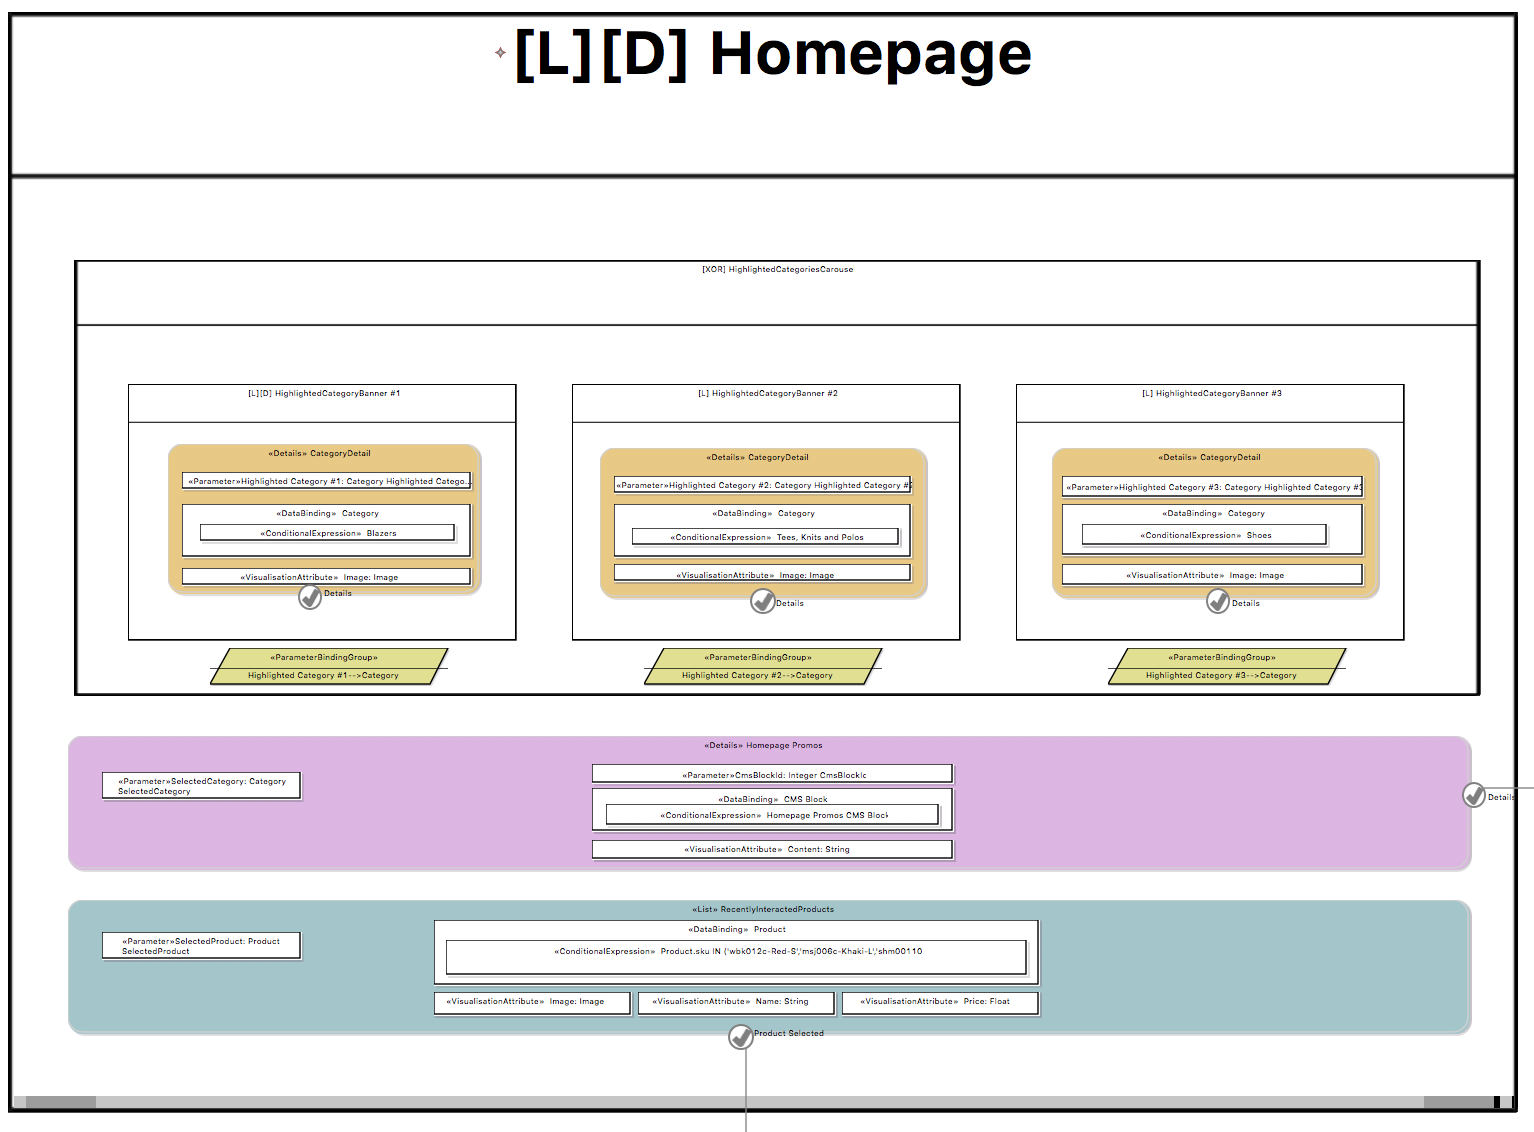
\includegraphics[height=9cm]{images/diagrams/after/ifml-homepage.png}
  \caption{Updated Homepage IFML Diagram}
  \label{fig:ifml-after-homepage}
\end{figure}

\begin{figure}[H]
  \centering
    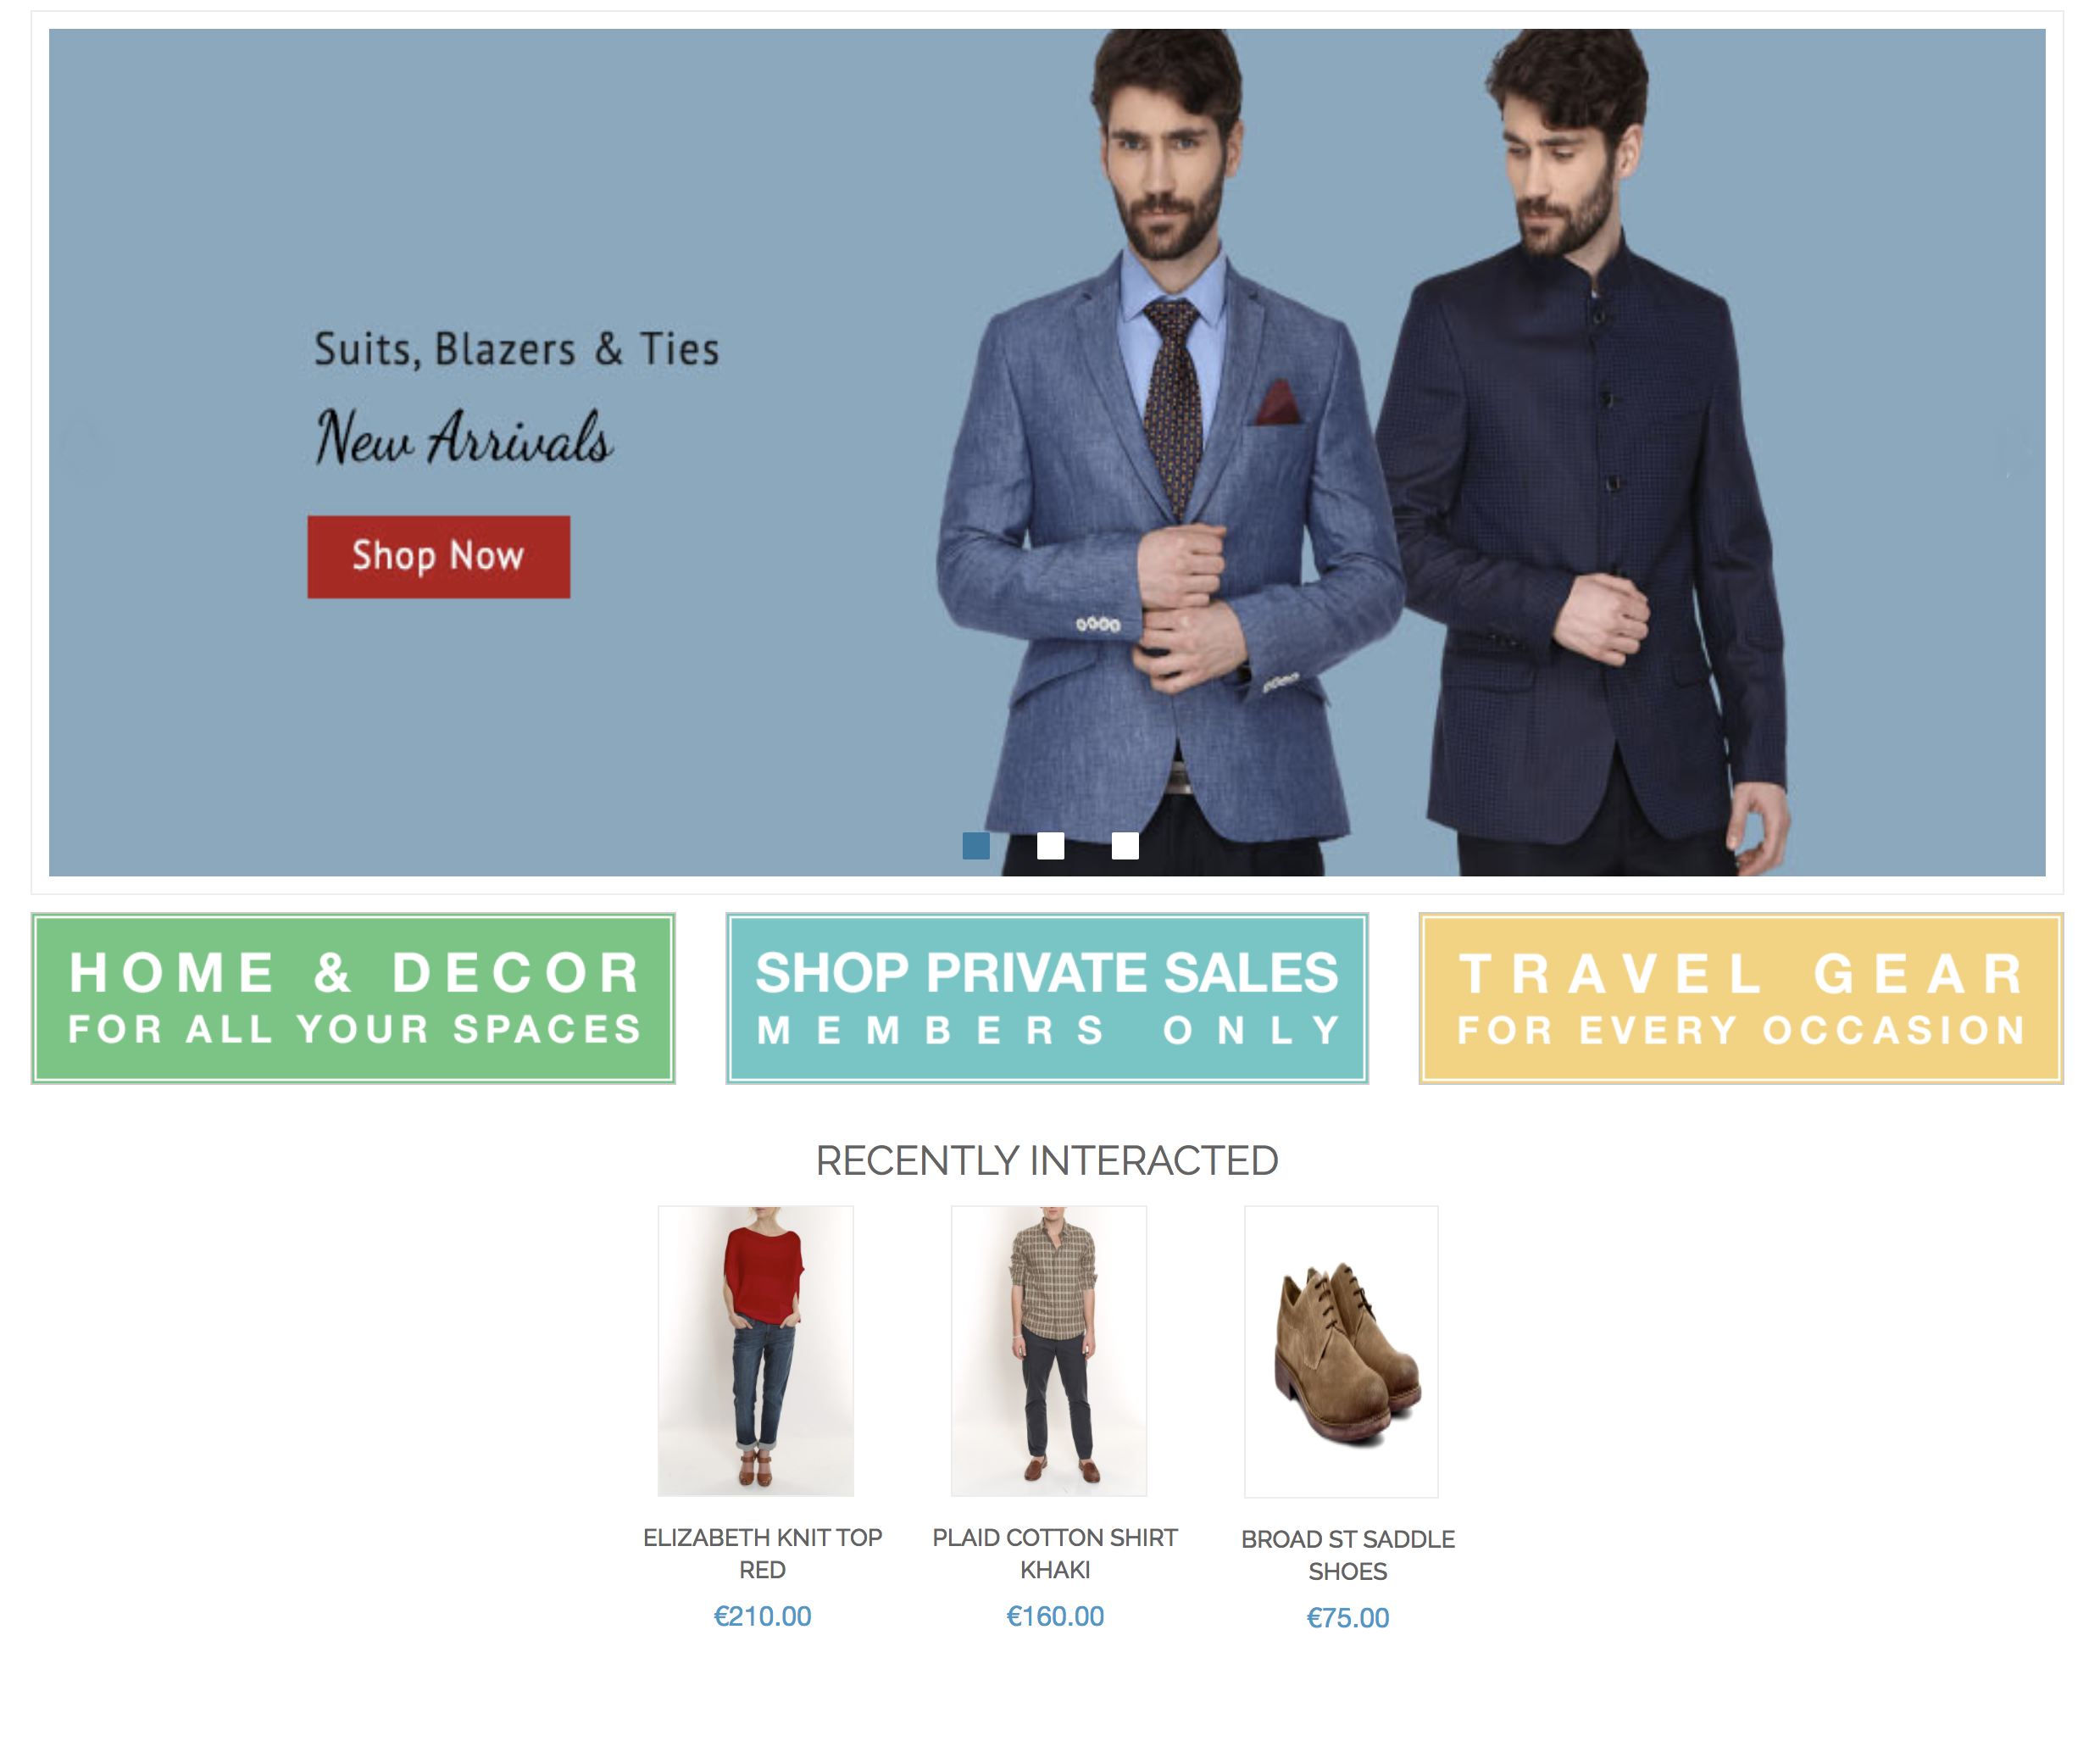
\includegraphics[height=9cm]{images/diagrams/after/desktop-homepage.png}
  \caption{Updated Homepage Desktop}
  \label{fig:desktop-before-homepage}
\end{figure}
\vspace{0.5cm}

\newpage
\subsection{Header}

After transforming its IFMLModel component (\ref{header-updates}), the shared header section on the website reveals new information through a new widget aligned on the right side of the area for advertising the actions the user made in the real world with the corresponding earned reward points.

\vspace{0.5cm}
\begin{figure}[H]
  \centering
    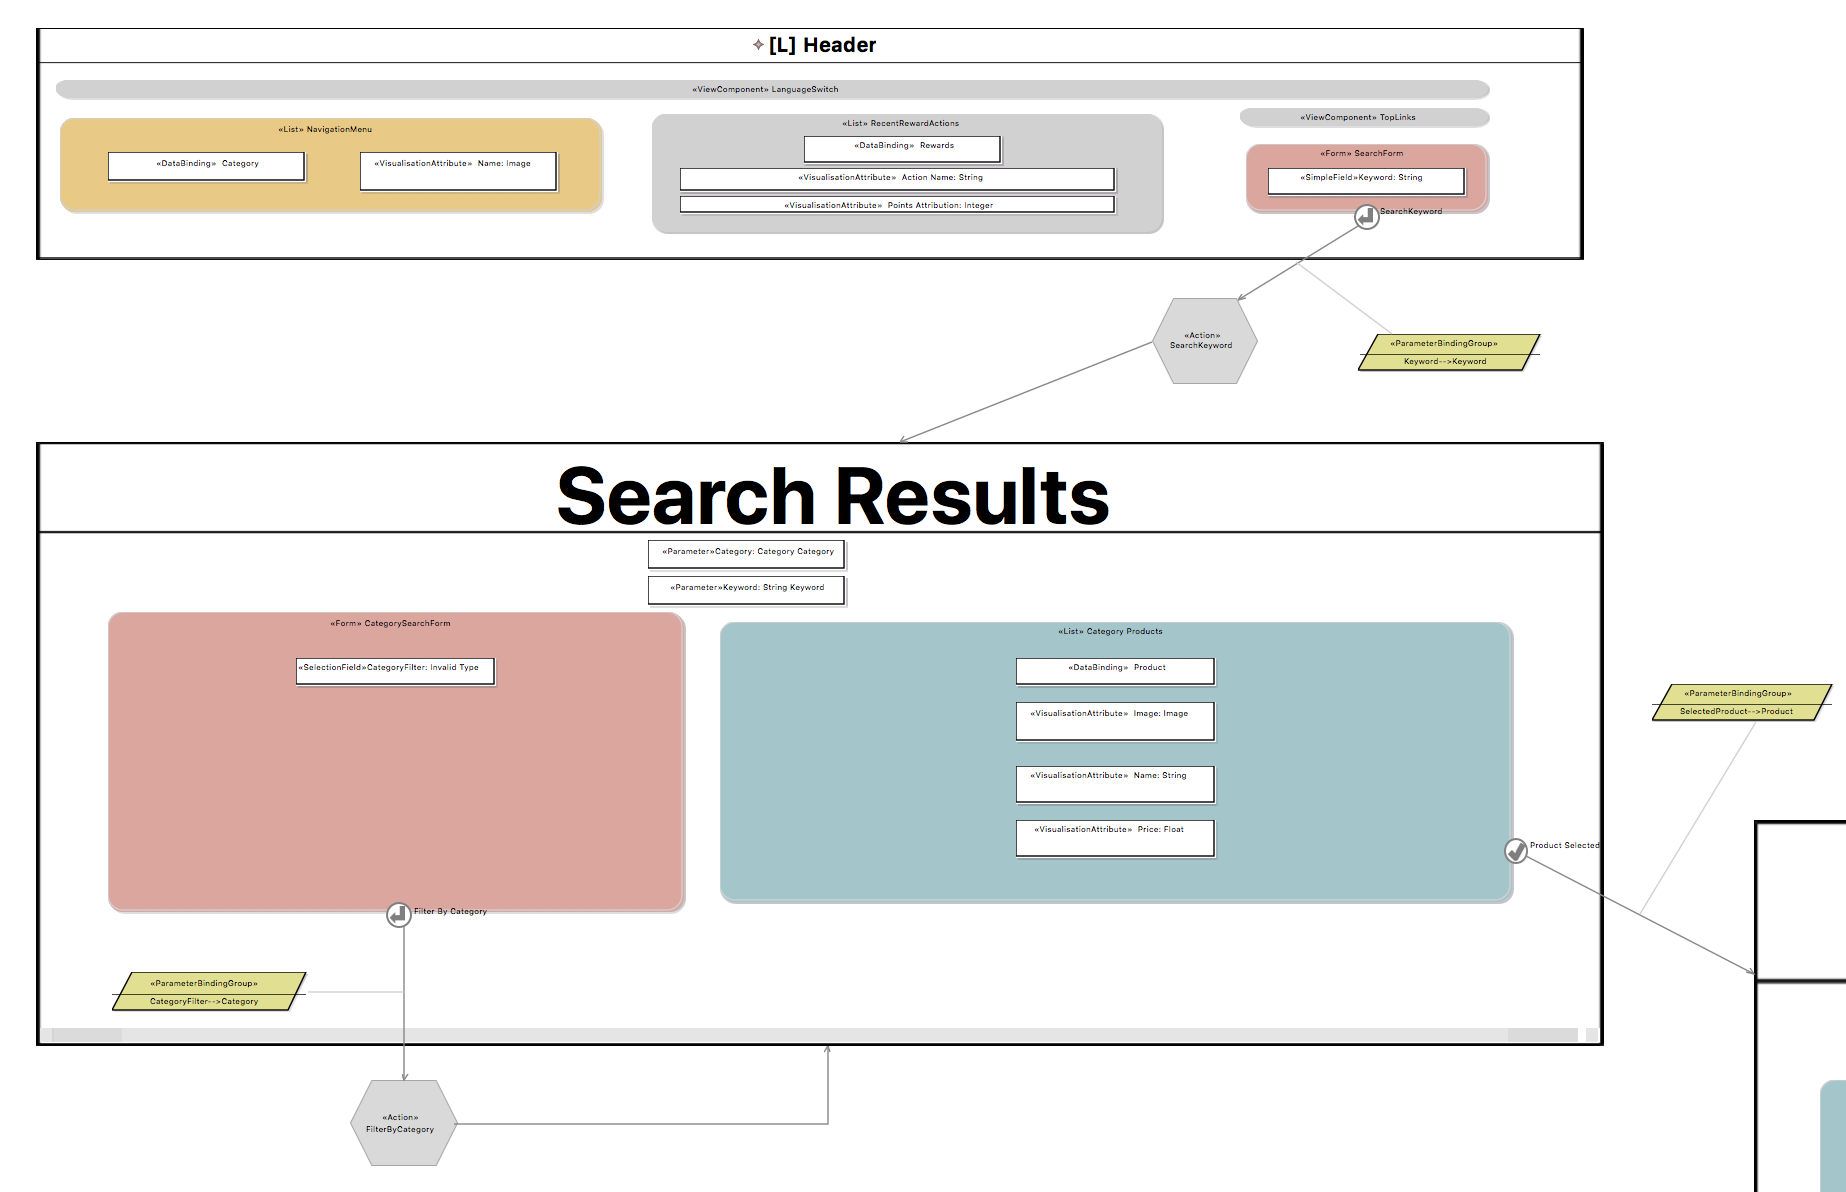
\includegraphics[width=14cm]{images/diagrams/after/ifml-header.png}
  \caption{Updated Header IFML Diagram}
  \label{fig:ifml-after-homepage}
\end{figure}

\begin{figure}[H]
  \centering
    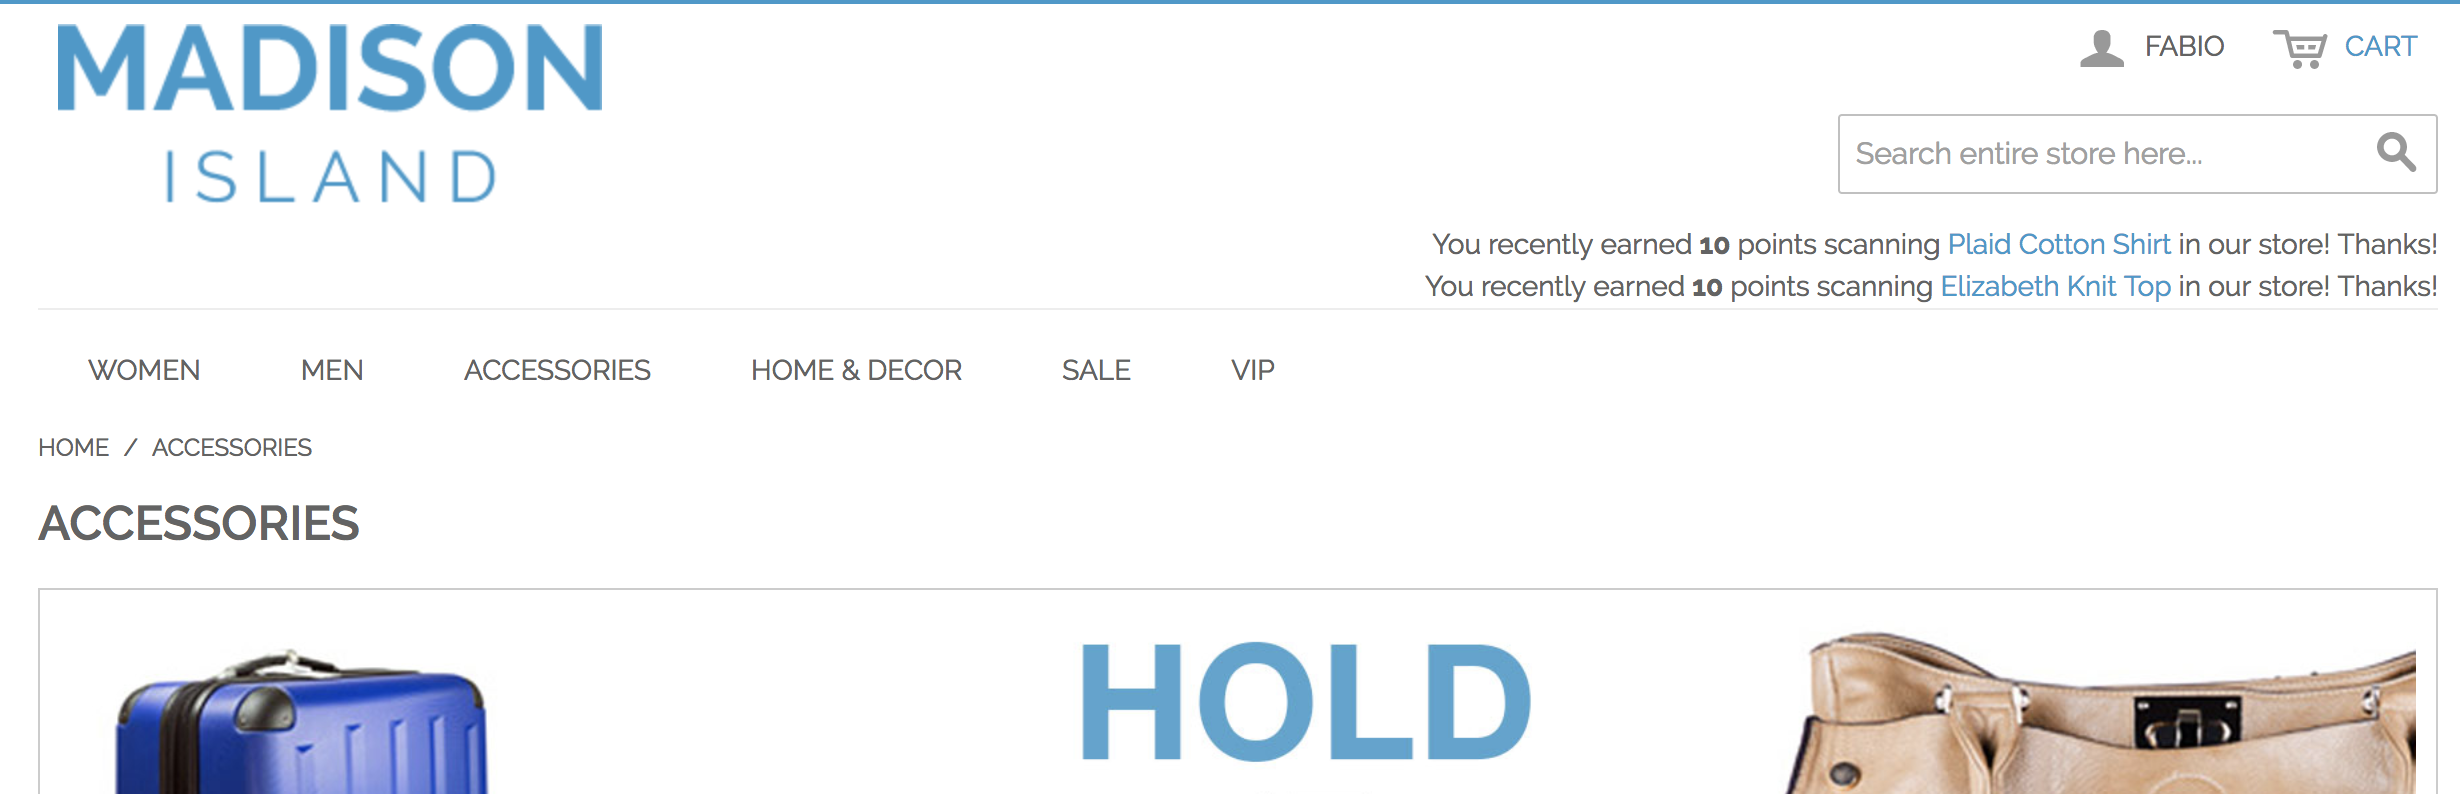
\includegraphics[width=14cm]{images/diagrams/after/desktop-header.png}
  \caption{Updated Header Desktop Version}
  \label{fig:desktop-after-header}
\end{figure}
\vspace{0.5cm}

\newpage
\subsection{Category Page}

Regardless of the DisplayMode property set for each Category Page, the updated web model presents a vertical section on the right sidebar which maps the recently browsed URLs recorded in the same user session which have been identified during the model transformation phase (\ref{category-page-updates}).

\vspace{0.5cm}
\begin{figure}[H]
  \centering
    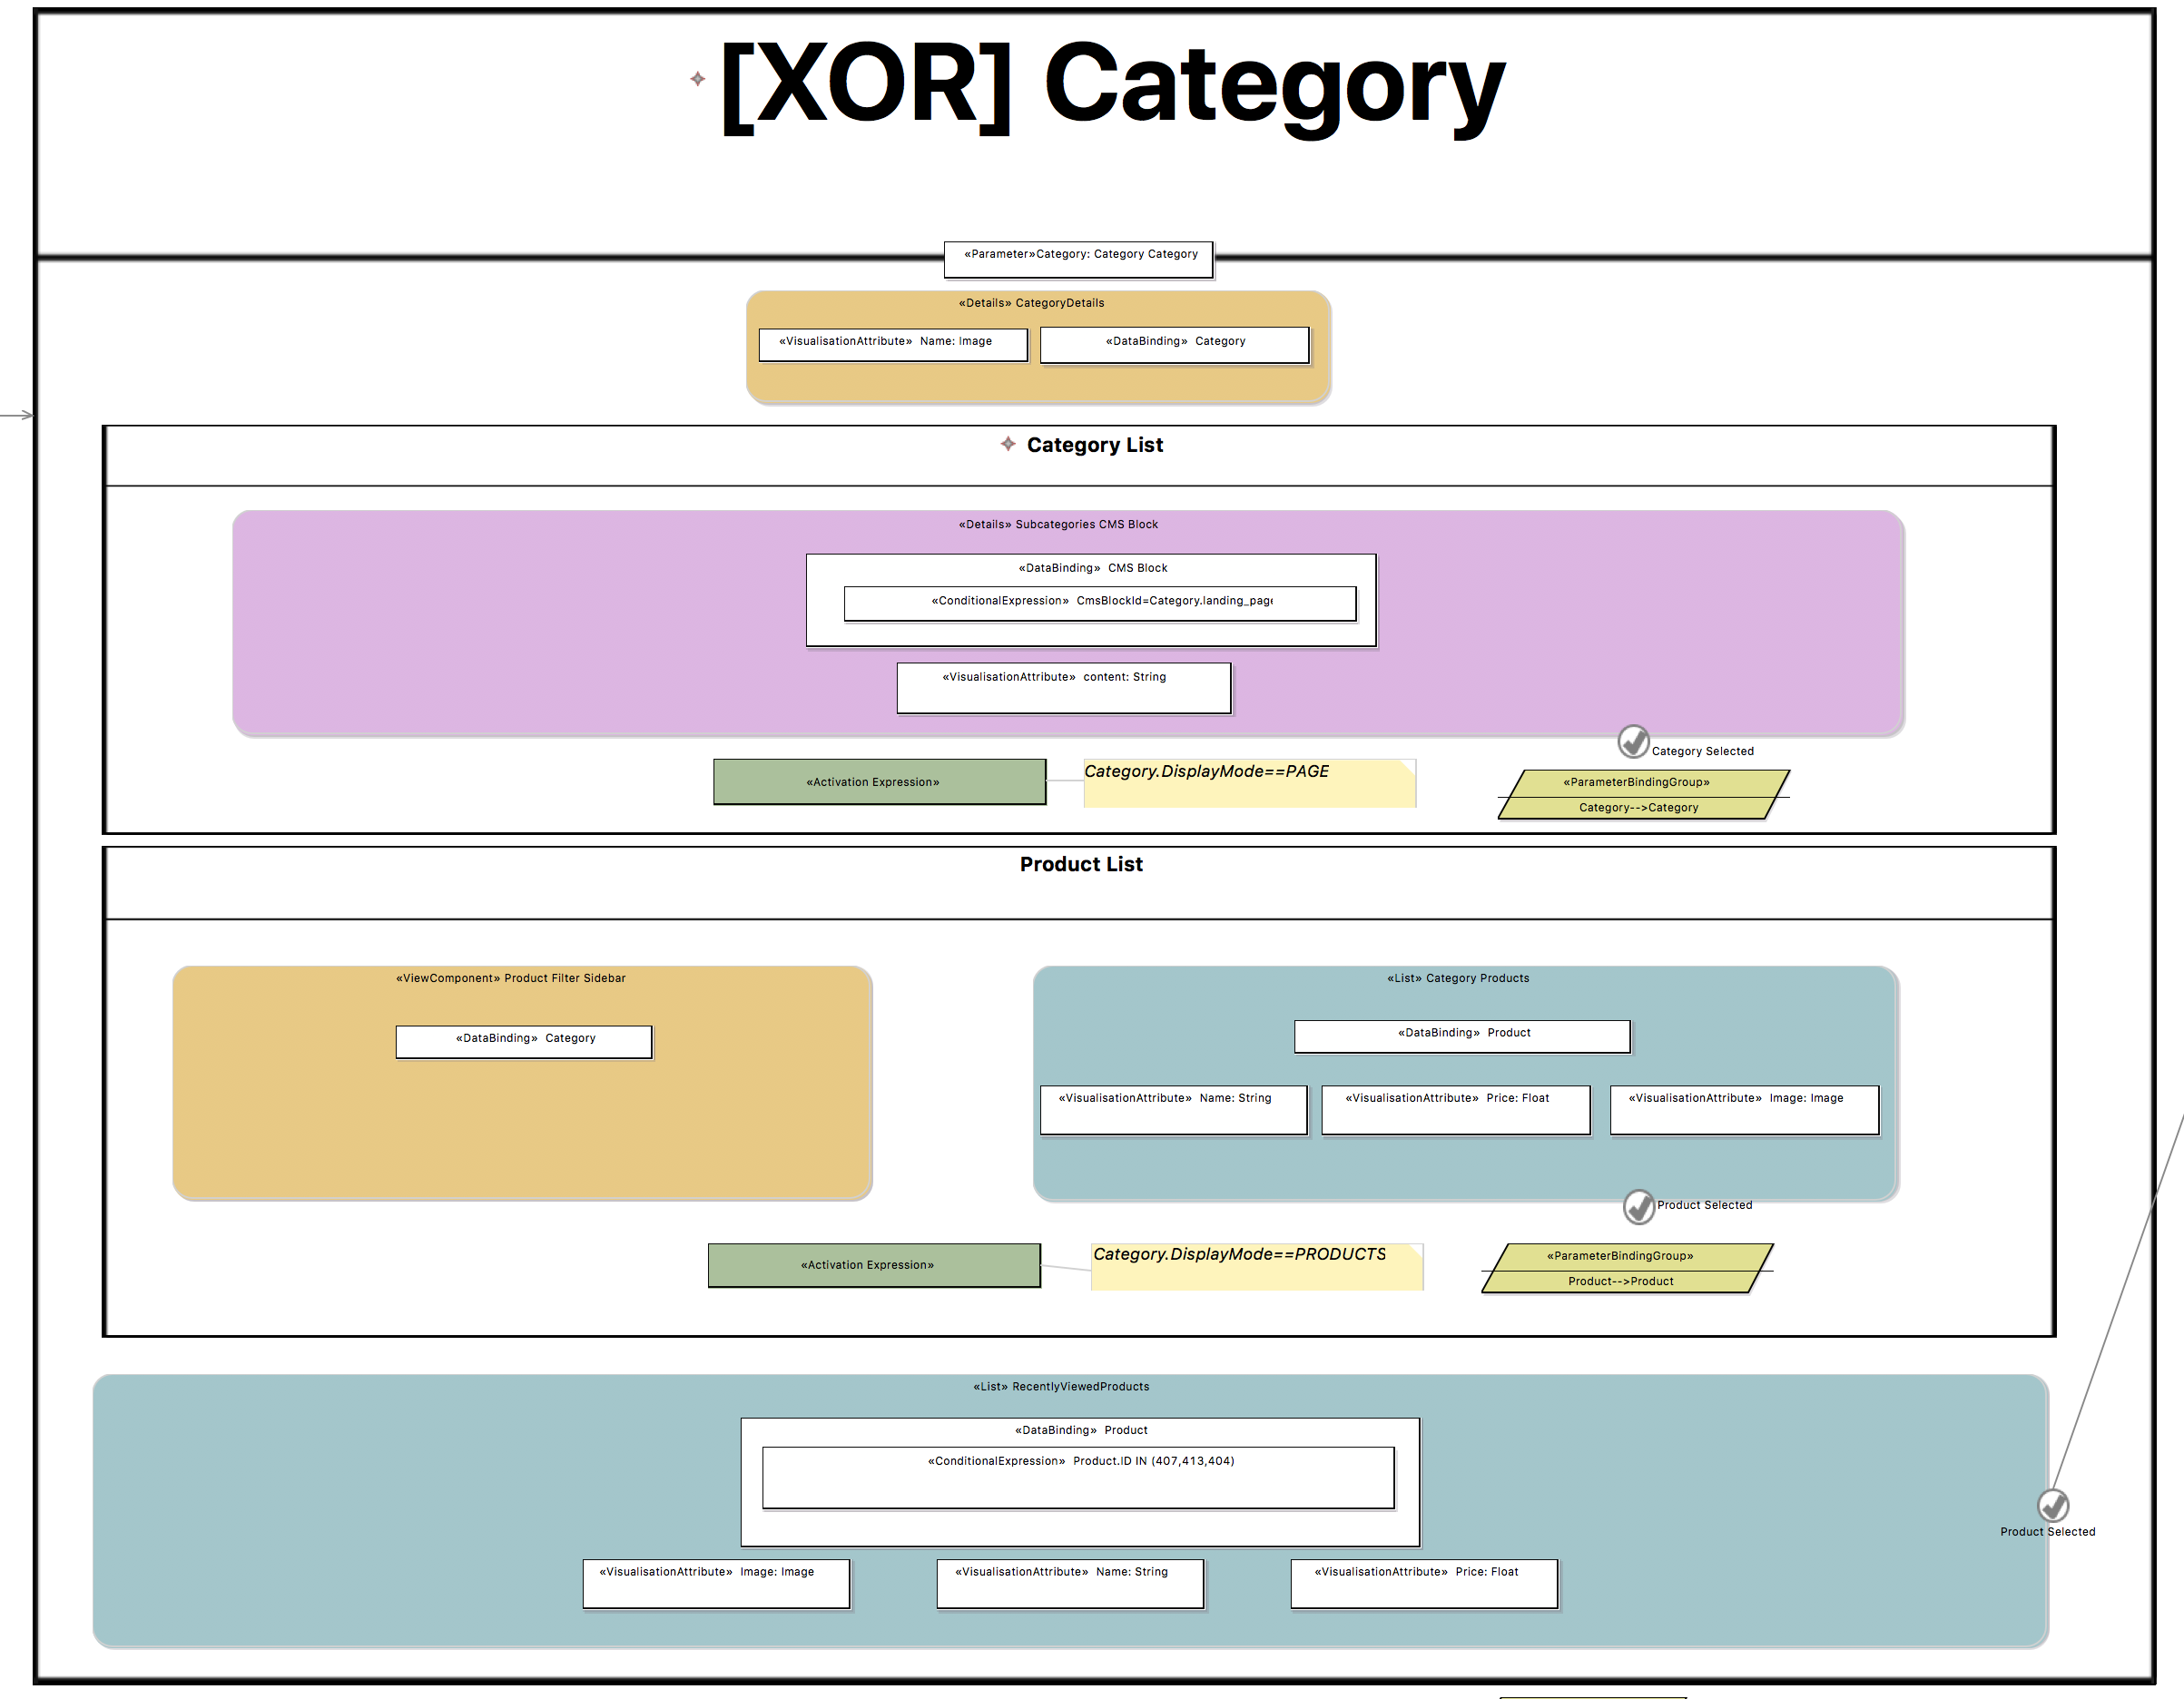
\includegraphics[height=12cm]{images/diagrams/after/ifml-category.png}
  \caption{Updated Category Page IFML Diagram}
  \label{fig:ifml-after-category}
\end{figure}

\begin{figure}[H]
  \centering
    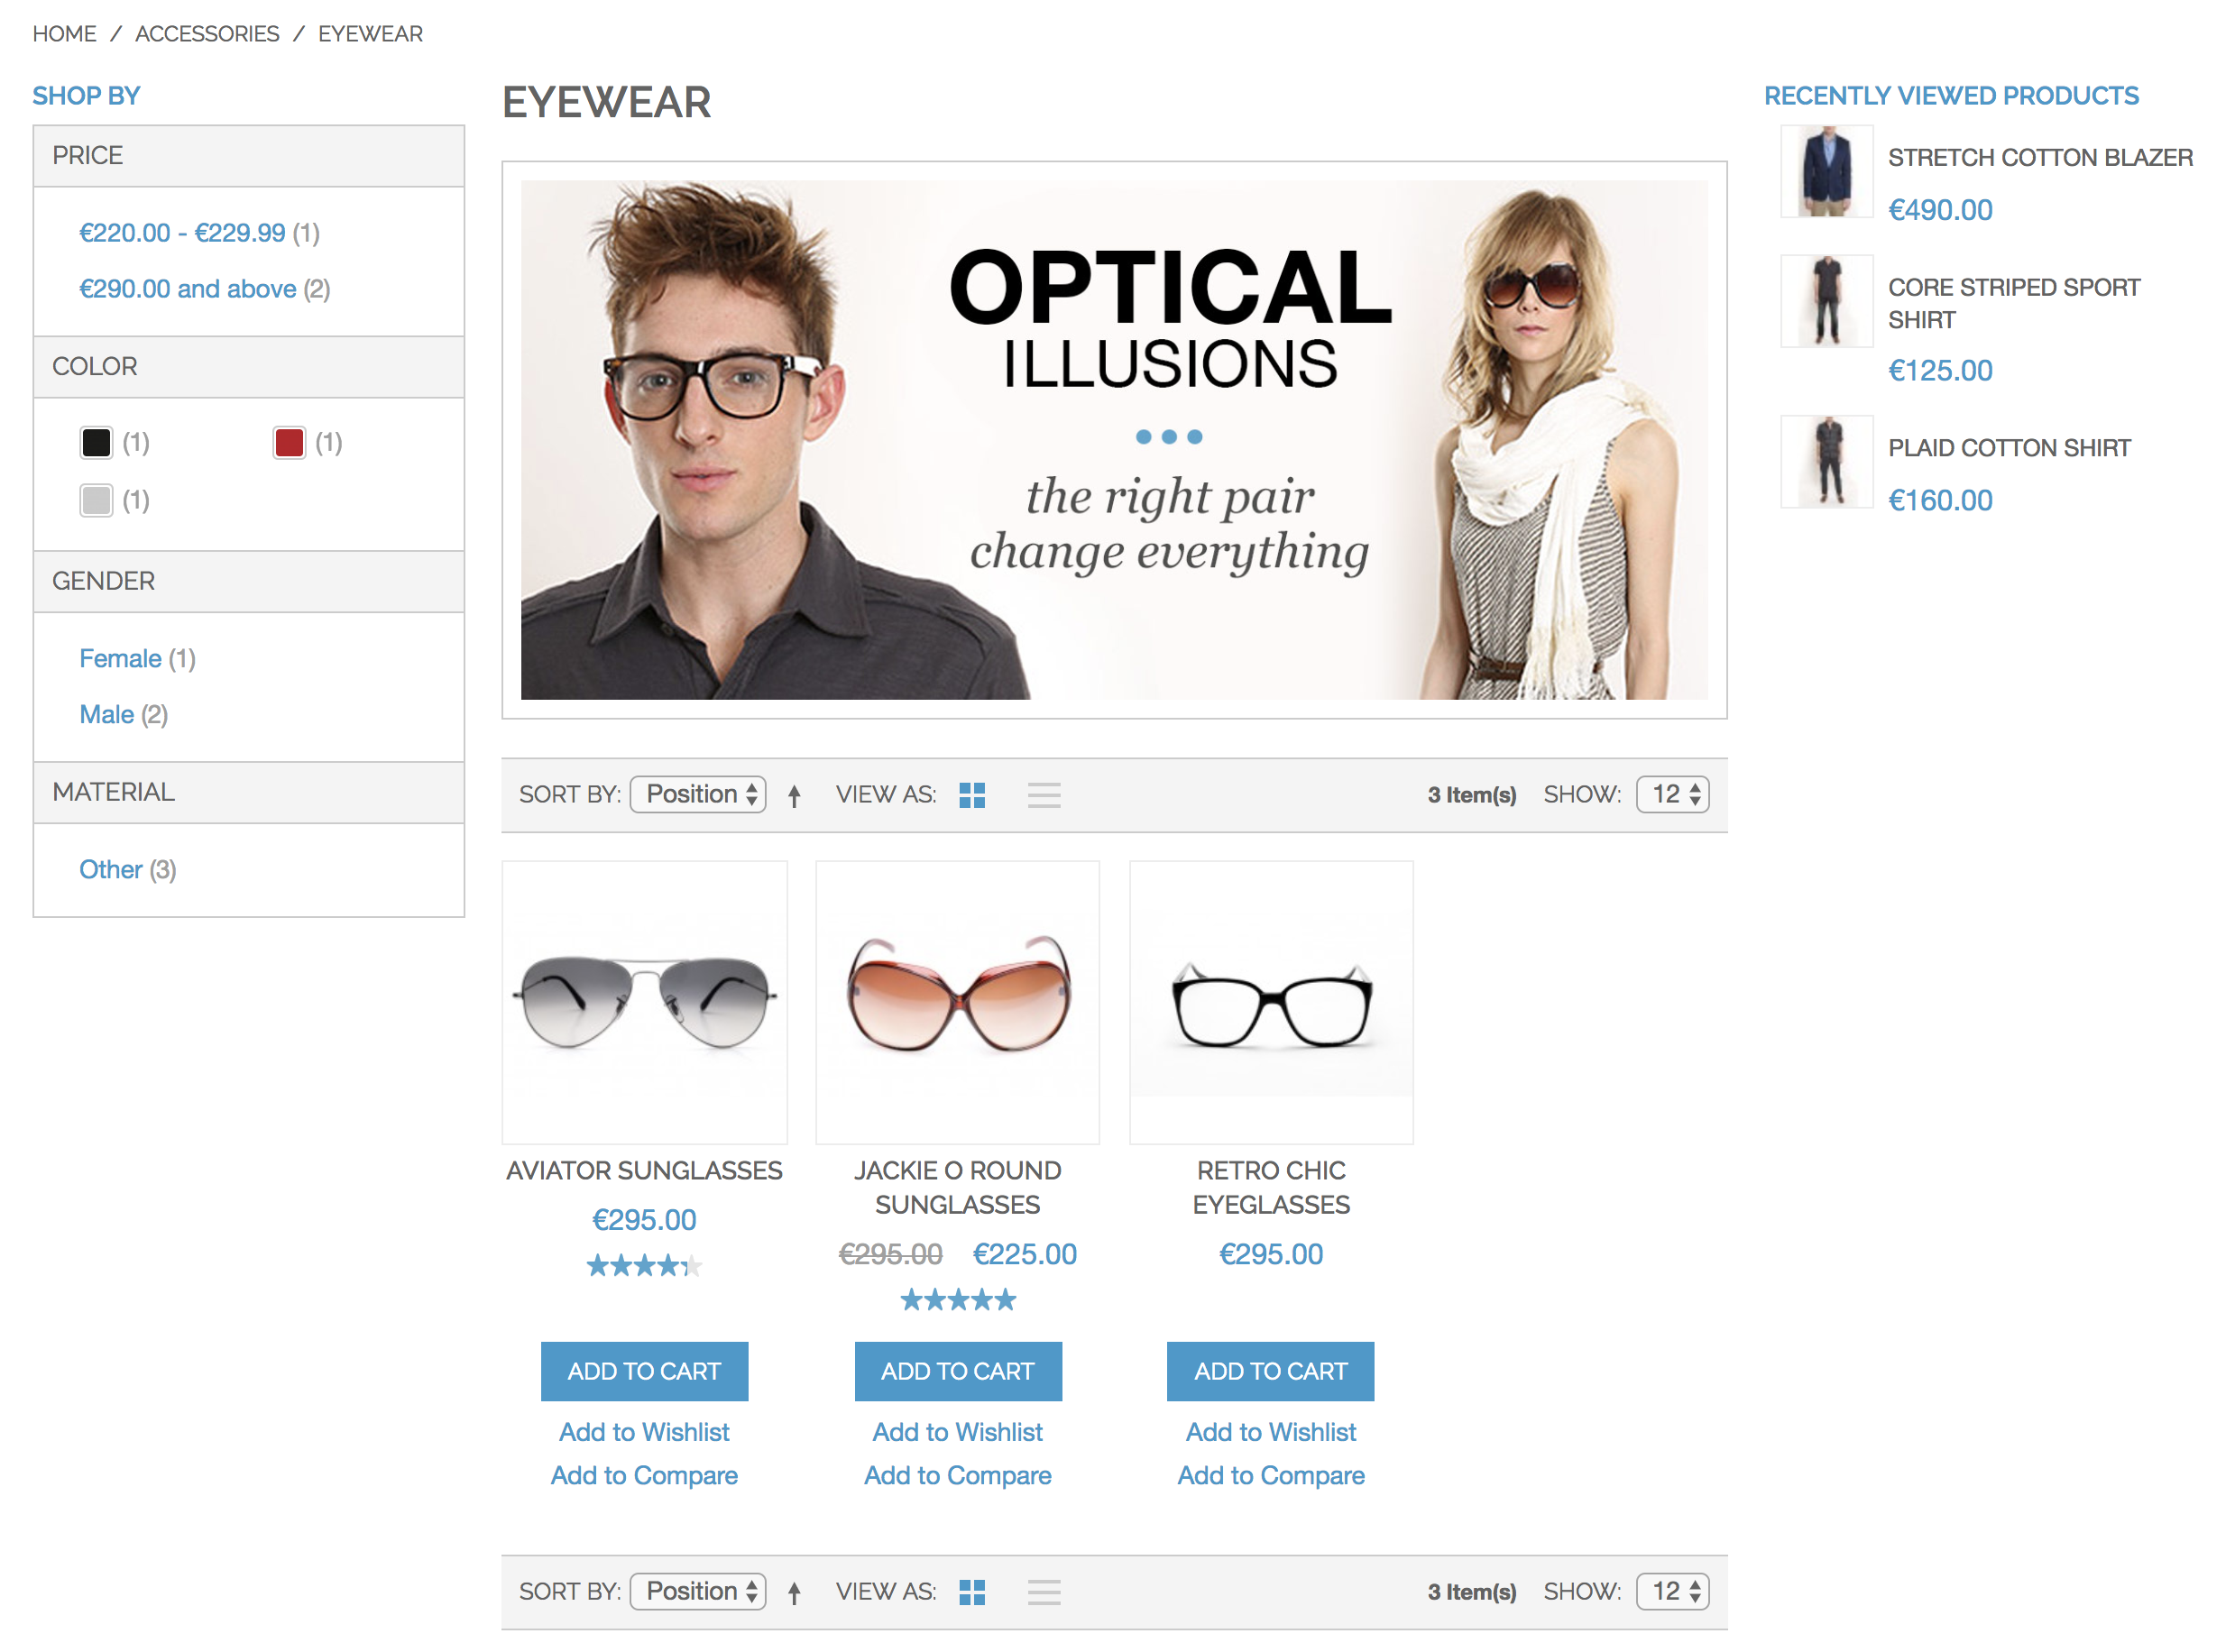
\includegraphics[height=12cm]{images/diagrams/after/desktop-category.png}
  \caption{Updated Category Page Desktop Version}
  \label{fig:desktop-after-category}
\end{figure}
\vspace{0.5cm}

\subsection{Product Page}

\subsection{Shopping Cart}

%\addcontentsline{toc}{chapter}{}